%%
%% This is file `sample-sigconf-authordraft.tex',
%% generated with the docstrip utility.
%%
%% The original source files were:
%%
%% samples.dtx  (with options: `all,proceedings,bibtex,authordraft')
%% 
%% IMPORTANT NOTICE:
%% 
%% For the copyright see the source file.
%% 
%% Any modified versions of this file must be renamed
%% with new filenames distinct from sample-sigconf-authordraft.tex.
%% 
%% For distribution of the original source see the terms
%% for copying and modification in the file samples.dtx.
%% 
%% This generated file may be distributed as long as the
%% original source files, as listed above, are part of the
%% same distribution. (The sources need not necessarily be
%% in the same archive or directory.)
%%
%%
%% Commands for TeXCount
%TC:macro \cite [option:text,text]
%TC:macro \citep [option:text,text]
%TC:macro \citet [option:text,text]
%TC:envir table 0 1
%TC:envir table* 0 1
%TC:envir tabular [ignore] word
%TC:envir displaymath 0 word
%TC:envir math 0 word
%TC:envir comment 0 0
%%
%% The first command in your LaTeX source must be the \documentclass
%% command.
%%
%% For submission and review of your manuscript please change the
%% command to \documentclass[manuscript, screen, review]{acmart}.
%%
%% When submitting camera ready or to TAPS, please change the command
%% to \documentclass[sigconf]{acmart} or whichever template is required
%% for your publication.
%%
%%
%\documentclass[sigconf,authordraft]{acmart}
\documentclass[sigconf,review,anonymous]{acmart}
%%
%% \BibTeX command to typeset BibTeX logo in the docs
\AtBeginDocument{%
  \providecommand\BibTeX{{%
    Bib\TeX}}}

%% Rights management information.  This information is sent to you
%% when you complete the rights form.  These commands have SAMPLE
%% values in them; it is your responsibility as an author to replace
%% the commands and values with those provided to you when you
%% complete the rights form.
\setcopyright{acmlicensed}
\copyrightyear{2018}
\acmYear{2018}
\acmDOI{XXXXXXX.XXXXXXX}
%% These commands are for a PROCEEDINGS abstract or paper.
\acmConference[Conference acronym 'XX]{Make sure to enter the correct
  conference title from your rights confirmation email}{June 03--05,
  2018}{Woodstock, NY}
%%
%%  Uncomment \acmBooktitle if the title of the proceedings is different
%%  from ``Proceedings of ...''!
%%
%%\acmBooktitle{Woodstock '18: ACM Symposium on Neural Gaze Detection,
%%  June 03--05, 2018, Woodstock, NY}
\acmISBN{978-1-4503-XXXX-X/2018/06}


%%
%% Submission ID.
%% Use this when submitting an article to a sponsored event. You'll
%% receive a unique submission ID from the organizers
%% of the event, and this ID should be used as the parameter to this command.
%%\acmSubmissionID{123-A56-BU3}

%%
%% For managing citations, it is recommended to use bibliography
%% files in BibTeX format.
%%
%% You can then either use BibTeX with the ACM-Reference-Format style,
%% or BibLaTeX with the acmnumeric or acmauthoryear sytles, that include
%% support for advanced citation of software artefact from the
%% biblatex-software package, also separately available on CTAN.
%%
%% Look at the sample-*-biblatex.tex files for templates showcasing
%% the biblatex styles.
%%

%%
%% The majority of ACM publications use numbered citations and
%% references.  The command \citestyle{authoryear} switches to the
%% "author year" style.
%%
%% If you are preparing content for an event
%% sponsored by ACM SIGGRAPH, you must use the "author year" style of
%% citations and references.
%% Uncommenting
%% the next command will enable that style.
%%\citestyle{acmauthoryear}
\usepackage{booktabs} % For formal tables
\usepackage{multirow}
\usepackage{graphicx}
\usepackage{subcaption}
\usepackage{tikz}
\usetikzlibrary{positioning, shapes.geometric, arrows.meta, fit, backgrounds, calc}
%\usepackage{amsmath,amssymb}

\usepackage{amsmath}
\let\Bbbk\relax
\usepackage{amssymb}

%%
%% end of the preamble, start of the body of the document source.
\begin{document}

%%
%% The "title" command has an optional parameter,
%% allowing the author to define a "short title" to be used in page headers.
\title{QUEST-KG: Evidence-Aware and Uncertainty-Calibrated Graph-RAG for Trustworthy Knowledge Graph Reasoning}


%%
%% The "author" command and its associated commands are used to define
%% the authors and their affiliations.
%% Of note is the shared affiliation of the first two authors, and the
%% "authornote" and "authornotemark" commands
%% used to denote shared contribution to the research.
\author{Ben Trovato}
\authornote{Both authors contributed equally to this research.}
\email{trovato@corporation.com}
\orcid{1234-5678-9012}
\author{G.K.M. Tobin}
\authornotemark[1]
\email{webmaster@marysville-ohio.com}
\affiliation{%
  \institution{Institute for Clarity in Documentation}
  \city{Dublin}
  \state{Ohio}
  \country{USA}
}

\author{Lars Th{\o}rv{\"a}ld}
\affiliation{%
  \institution{The Th{\o}rv{\"a}ld Group}
  \city{Hekla}
  \country{Iceland}}
\email{larst@affiliation.org}

\author{Valerie B\'eranger}
\affiliation{%
  \institution{Inria Paris-Rocquencourt}
  \city{Rocquencourt}
  \country{France}
}

\author{Aparna Patel}
\affiliation{%
 \institution{Rajiv Gandhi University}
 \city{Doimukh}
 \state{Arunachal Pradesh}
 \country{India}}

\author{Huifen Chan}
\affiliation{%
  \institution{Tsinghua University}
  \city{Haidian Qu}
  \state{Beijing Shi}
  \country{China}}

\author{Charles Palmer}
\affiliation{%
  \institution{Palmer Research Laboratories}
  \city{San Antonio}
  \state{Texas}
  \country{USA}}
\email{cpalmer@prl.com}

\author{John Smith}
\affiliation{%
  \institution{The Th{\o}rv{\"a}ld Group}
  \city{Hekla}
  \country{Iceland}}
\email{jsmith@affiliation.org}

\author{Julius P. Kumquat}
\affiliation{%
  \institution{The Kumquat Consortium}
  \city{New York}
  \country{USA}}
\email{jpkumquat@consortium.net}

%%
%% By default, the full list of authors will be used in the page
%% headers. Often, this list is too long, and will overlap
%% other information printed in the page headers. This command allows
%% the author to define a more concise list
%% of authors' names for this purpose.
\renewcommand{\shortauthors}{Trovato et al.}

%%
%% The abstract is a short summary of the work to be presented in the
%% article.

\begin{abstract}

Knowledge graphs (KGs) increasingly support enterprise intelligence, retrieval-augmented reasoning, policy enforcement, and multi-hop question answering across heterogeneous and evolving data ecosystems. However, existing KG reasoning systems often optimize predictive accuracy while providing limited support for provenance-aware inference, calibrated uncertainty estimation, and robust reasoning under incomplete, noisy, or dynamically changing evidence. These limitations become particularly critical in cross-domain and security-sensitive environments where trustworthy, auditable, and evidence-grounded reasoning is required.
We present \textbf{QUEST-KG}, an evidence-aware and uncertainty-calibrated Graph-RAG framework for trustworthy knowledge graph reasoning. QUEST-KG unifies symbolic graph structure, semantic retrieval, provenance-aware evidential fusion, and neuro-symbolic reasoning within a single interpretable inference pipeline. The framework integrates: (1) a schema-aware Graph-RAG retrieval layer for grounded subgraph construction; (2) an evidential message-passing mechanism that propagates calibrated belief and uncertainty across multi-hop reasoning chains; and (3) a provenance-linked neuro-symbolic reasoning module for dynamic policy and access-control inference. Unlike conventional end-to-end neural reasoning systems, QUEST-KG explicitly models evidence reliability, uncertainty propagation, and semantic consistency during inference, enabling transparent, auditable decision-making.
We evaluate QUEST-KG across three representative reasoning settings: cross-lingual entity alignment, multi-hop question answering, and dynamic knowledge-graph access control. Experiments on IDS100K, DWY100K, WebQSP, ComplexWebQuestions, ICEWS18, and OrgAccess demonstrate that QUEST-KG achieves highly competitive or state-of-the-art performance while substantially improving calibration, robustness, and reasoning transparency compared with neural, symbolic, retrieval-augmented, and agentic baselines. Additional analyses show that provenance-aware evidential fusion improves robustness under structural incompleteness and noisy retrieval conditions while maintaining efficient inference latency suitable for real-world deployment.
These results suggest that evidence-aware, uncertainty-calibrated Graph-RAG reasoning provides a scalable, trustworthy foundation for next-generation knowledge-centric AI systems operating over heterogeneous, evolving knowledge graphs.

\end{abstract}

%%
%% The code below is generated by the tool at http://dl.acm.org/ccs.cfm.
%% Please copy and paste the code instead of the example below.
%%
\begin{CCSXML}
<ccs2012>
 <concept>
  <concept_id>10002951.10003317.10003359.10003360</concept_id>
  <concept_desc>Information systems~Ontology engineering</concept_desc>
  <concept_significance>500</concept_significance>
 </concept>
 <concept>
  <concept_id>10002951.10003317.10003347.10003350</concept_id>
  <concept_desc>Information systems~Information extraction</concept_desc>
  <concept_significance>300</concept_significance>
 </concept>
 <concept>
  <concept_id>10010147.10010257.10010258.10010259.10010263</concept_id>
  <concept_desc>Computing methodologies~Knowledge representation and reasoning</concept_desc>
  <concept_significance>300</concept_significance>
 </concept>
 <concept>
  <concept_id>10010147.10010257.10010293.10010294</concept_id>
  <concept_desc>Computing methodologies~Neural networks</concept_desc>
  <concept_significance>100</concept_significance>
 </concept>
 <concept>
  <concept_id>10002951.10003317.10003338</concept_id>
  <concept_desc>Information systems~Retrieval models and ranking</concept_desc>
  <concept_significance>100</concept_significance>
 </concept>
</ccs2012>
\end{CCSXML}

\ccsdesc[500]{Information systems~Ontology engineering}
\ccsdesc[300]{Information systems~Information extraction}
\ccsdesc[300]{Computing methodologies~Knowledge representation and reasoning}
\ccsdesc[100]{Computing methodologies~Neural networks}
\ccsdesc[100]{Information systems~Retrieval models and ranking}

%%
%% Keywords
\keywords{
knowledge graphs,
Graph-RAG,
evidential reasoning,
uncertainty calibration,
neuro-symbolic reasoning,
provenance-aware inference,
multi-hop question answering,
entity alignment,
trustworthy AI,
knowledge graph retrieval,
access control reasoning,
retrieval-augmented reasoning
}
%%
%% Remove ACM sample received dates for submission version
% \received{20 February 2007}
% \received[revised]{12 March 2009}
% \received[accepted]{5 June 2009}
%%
%% This command processes the author and affiliation and title
%% information and builds the first part of the formatted document.
\maketitle
\section{Introduction}

Knowledge graphs (KGs) have become a foundational infrastructure for modern information systems and knowledge-centric AI, enabling semantic search, multi-hop reasoning, enterprise intelligence, and retrieval-augmented generation (RAG) across heterogeneous data ecosystems~\cite{hogan2021knowledge,ji2022survey}. Recent advances in large language models (LLMs) and retrieval-augmented reasoning have further accelerated interest in graph-centric retrieval pipelines that combine symbolic relational structure with neural semantic retrieval~\cite{lewis2020retrieval}. Compared with conventional vector-based retrieval, graph-aware retrieval better preserves relational dependencies, supports compositional reasoning, and provides interpretable evidence aggregation for knowledge-intensive tasks such as question answering, entity alignment, and policy reasoning~\cite{ren2020query2box,ren2020betae}. Recent GraphRAG research further highlights the growing importance of graph-structured retrieval for context-aware and multi-hop reasoning in knowledge-intensive AI systems.

Despite rapid progress, existing Graph-RAG and KG reasoning systems still face major challenges in trustworthy reasoning, uncertainty calibration, and provenance-aware inference. Many current approaches rely on opaque end-to-end neural pipelines that optimize predictive accuracy while providing limited support for calibrated confidence estimation, explicit evidence tracing, or robust reasoning under incomplete, noisy, and evolving graph structures. These limitations become particularly problematic in enterprise and security-sensitive environments where reasoning systems must operate over heterogeneous, partially conflicting, and dynamically evolving knowledge sources. In such settings, reliable reasoning requires more than accurate retrieval: systems must reconcile conflicting evidence, quantify uncertainty, preserve provenance, and generate interpretable reasoning traces.

Recent studies further suggest that retrieval quality alone does not guarantee reliable downstream reasoning. Even when relevant evidence is successfully retrieved, neural reasoning systems often exhibit overconfident predictions, unstable multi-hop reasoning behavior, and brittle inference under schema drift or missing relational context. Similarly, uncertainty-aware graph reasoning research has emphasized the importance of explicitly modeling epistemic uncertainty, evidence reliability, and confidence calibration during graph inference rather than relying solely on larger language models or improved embeddings. These observations motivate integrated reasoning frameworks that jointly support evidence-aware graph retrieval, uncertainty-calibrated reasoning, provenance-aware inference, and interpretable multi-hop reasoning under incomplete and evolving graph structures.

To address these challenges, we introduce \textbf{QUEST-KG}, an evidence-aware and uncertainty-calibrated Graph-RAG framework for trustworthy knowledge graph reasoning. The central idea of QUEST-KG is to treat graph retrieval and downstream reasoning as a unified evidential inference process with explicit uncertainty propagation and provenance-aware belief fusion. Unlike conventional Graph-RAG pipelines that treat retrieval and reasoning as largely independent stages, QUEST-KG propagates provenance-weighted evidential uncertainty directly over retrieved subgraphs during multi-hop inference. Rather than separating retrieval, reasoning, and calibration into disconnected components, QUEST-KG integrates symbolic graph structure, semantic retrieval, provenance-aware evidential fusion, and neuro-symbolic reasoning within a single interpretable reasoning pipeline.

QUEST-KG combines three tightly integrated components: (i) a schema-aware Graph-RAG retrieval layer for grounded and semantically consistent subgraph construction, (ii) a provenance-aware evidential message-passing mechanism for calibrated belief propagation and uncertainty estimation, and (iii) a neuro-symbolic reasoning module that combines symbolic constraints with graph-based neural inference for dynamic multi-hop reasoning. Unlike conventional end-to-end neural reasoning systems, QUEST-KG explicitly preserves provenance, semantic consistency, and uncertainty estimates throughout inference, enabling calibrated confidence estimation, selective abstention under insufficient evidence, and interpretable reasoning traces suitable for trustworthy and enterprise-scale AI systems.

We evaluate QUEST-KG across three representative graph reasoning settings: cross-lingual and cross-domain entity alignment, multi-hop question answering, and dynamic knowledge-graph access-control reasoning. Experiments on IDS100K, DWY100K, WebQSP, ComplexWebQuestions, ICEWS18, and OrgAccess demonstrate that QUEST-KG achieves strong empirical performance while improving calibration, robustness, and reasoning transparency compared with neural, symbolic, retrieval-augmented, and agentic baselines. Additional analyses show that provenance-aware evidential fusion improves robustness under noisy retrieval conditions, missing relational structure, and evolving graph contexts while maintaining efficient inference latency suitable for real-world deployment.

The main contributions of this work are summarized as follows:

\begin{itemize}
    \item \textbf{Unified evidence-aware Graph-RAG framework.}
    We introduce QUEST-KG, a unified, evidence-aware, and uncertainty-calibrated Graph-RAG framework that integrates graph retrieval, provenance-aware reasoning, and uncertainty propagation into a single interpretable reasoning pipeline.

    \item \textbf{Provenance-aware evidential reasoning.}
    We propose a provenance-aware evidential message-passing mechanism that jointly models belief propagation, semantic consistency, and uncertainty calibration during multi-hop graph reasoning over incomplete and evolving graph structures.

    \item \textbf{Neuro-symbolic graph reasoning.}
    We develop a neuro-symbolic reasoning framework that combines symbolic graph constraints with retrieval-augmented neural inference to support interpretable, robust reasoning in noisy, heterogeneous graph environments.

    \item \textbf{Comprehensive evaluation across multiple graph reasoning tasks.}
    We conduct extensive experiments across cross-lingual entity alignment, multi-hop question answering, and dynamic access-control reasoning benchmarks, demonstrating improvements in robustness, calibration, interpretability, and retrieval-grounded reasoning quality.
\end{itemize}

Our results suggest that evidence-aware Graph-RAG reasoning with explicit uncertainty modeling and provenance-aware inference provides a scalable and trustworthy foundation for next-generation knowledge-centric AI systems operating over heterogeneous and evolving graph ecosystems.

\section{Related Work}

\subsection{Knowledge Graph Reasoning and Multi-Hop Inference}

Knowledge graph reasoning has become a central research direction in knowledge-centric AI and information systems. Early embedding-based approaches focused on relational representation learning and link prediction through translational and geometric embedding methods such as TransE~\cite{bordes2013transe}, RotatE~\cite{sun2019rotate}, Query2Box~\cite{ren2020query2box}, and BetaE~\cite{ren2020betae}. These methods demonstrated strong performance for compositional and multi-hop reasoning by embedding logical queries into continuous vector spaces. More recent approaches have incorporated graph neural networks (GNNs) and neural message passing to improve structural reasoning and contextual aggregation over large-scale knowledge graphs~\cite{schlichtkrull2018modeling,velivckovic2018graph}. 

Recent research has further explored query-guided graph reasoning and neuro-symbolic graph inference for complex question answering and retrieval-grounded reasoning~\cite{yao2021kagnn}. Despite substantial progress, many existing KG reasoning systems primarily optimize predictive accuracy while providing limited support for calibrated uncertainty estimation, provenance-aware reasoning, and interpretable evidence tracing. Furthermore, purely neural approaches often exhibit brittle behavior under schema drift, noisy graph structures, and incomplete relational evidence. These limitations motivate integrated frameworks that jointly support uncertainty-aware inference, symbolic consistency, and interpretable multi-hop reasoning.

\subsection{Retrieval-Augmented Generation and GraphRAG}

Retrieval-augmented generation (RAG) has emerged as an effective paradigm for improving factual grounding and knowledge access in large language models~\cite{lewis2020retrieval}. Conventional RAG systems primarily rely on dense vector retrieval over unstructured documents; however, recent studies have demonstrated that graph-structured retrieval can substantially improve compositional reasoning, contextual consistency, and interpretability for knowledge-intensive tasks~\cite{pan2024graphrag}. 

Recent GraphRAG frameworks combine graph traversal, semantic retrieval, and LLM-based reasoning to support context-aware retrieval over structured knowledge sources. Microsoft GraphRAG~\cite{edge2024graphrag} and related graph-centric retrieval frameworks demonstrate that structured graph retrieval can improve evidence aggregation and long-context reasoning compared with purely vector-based retrieval. Similarly, retrieval-grounded reasoning systems such as KG-Augmented Language Models and graph-guided QA frameworks have shown that integrating relational structure with neural retrieval improves multi-hop reasoning consistency and factual grounding~\cite{yao2021kagnn}. 

Nevertheless, most existing GraphRAG systems still treat retrieval and downstream reasoning as largely independent stages and provide limited support for uncertainty calibration, provenance-aware inference, and robust reasoning under incomplete and evolving graph structures. In contrast, QUEST-KG models retrieval and downstream reasoning as a unified evidential inference process with explicit uncertainty propagation and provenance-aware belief fusion.

\subsection{Uncertainty-Aware and Trustworthy Graph Reasoning}

Uncertainty estimation and trustworthy inference have become increasingly important for graph-based AI systems operating in noisy, heterogeneous, and dynamically evolving environments~\cite{chen2023trustworthy}. Existing research has explored Bayesian graph neural networks, evidential deep learning, calibration-aware inference, and probabilistic message passing for improving robustness and reliability under uncertainty~\cite{sensoy2018evidential,amini2020deep}. 

Recent trustworthy graph learning research emphasizes that predictive accuracy alone is insufficient for reliable deployment in enterprise and security-sensitive environments. Instead, graph reasoning systems must support calibrated confidence estimation, robustness to noisy evidence, and interpretable reasoning traces~\cite{liu2022trustworthy}. Although existing uncertainty-aware graph learning methods improve robustness for tasks such as node classification and link prediction, most do not explicitly integrate provenance-aware retrieval, symbolic reasoning constraints, and multi-hop evidential reasoning within a unified GraphRAG framework.

\subsection{Neuro-Symbolic Reasoning and Knowledge-Grounded AI}

Neuro-symbolic reasoning aims to combine the generalization capability of neural models with the interpretability and logical consistency of symbolic reasoning systems~\cite{garcez2019neural}. Recent work has explored neuro-symbolic approaches for question answering, graph reasoning, and knowledge-grounded inference by integrating symbolic constraints with neural retrieval and representation learning~\cite{mao2019neuro}. 

Knowledge-grounded reasoning frameworks have demonstrated that combining symbolic relational structure with neural inference improves reasoning consistency, interpretability, and compositional generalization for complex reasoning tasks~\cite{yao2021kagnn}. However, many existing systems still lack explicit mechanisms for provenance-aware evidence fusion and uncertainty-calibrated reasoning. Moreover, most prior work focuses on single-task settings such as question answering or logical inference. QUEST-KG extends this direction by integrating neuro-symbolic reasoning, provenance-aware evidential fusion, and uncertainty-calibrated GraphRAG retrieval within a unified framework applicable to entity alignment, multi-hop reasoning, and dynamic access-control inference.

\subsection{Positioning of QUEST-KG}

QUEST-KG differs from prior work in three important ways. First, unlike conventional GraphRAG pipelines that separate retrieval and downstream reasoning, QUEST-KG models retrieval and inference as a unified evidential reasoning process with explicit uncertainty propagation. Second, the framework integrates provenance-aware evidential message passing with neuro-symbolic graph reasoning to support calibrated and interpretable multi-hop inference under incomplete and evolving graph structures. Third, QUEST-KG provides a unified framework that supports multiple graph reasoning tasks, including entity alignment, multi-hop question answering, and dynamic access-control reasoning, while preserving semantic consistency, provenance, and uncertainty estimates throughout inference.

\section{Methodology}

\begin{figure*}[t]
\centering
\resizebox{0.98\textwidth}{!}{%
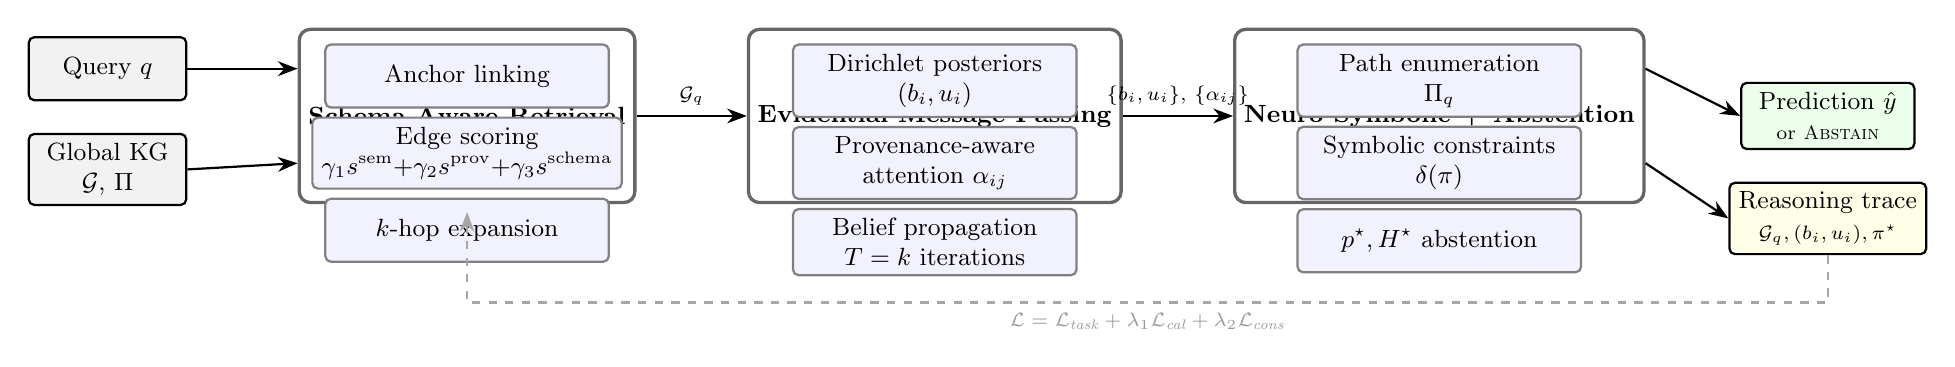
\begin{tikzpicture}[
  font=\small,
  node distance=8mm and 8mm,
  stage/.style={
    rectangle, rounded corners=4pt, draw=black!60, very thick,
    minimum width=42mm, minimum height=22mm, align=center, fill=white
  },
  module/.style={
    rectangle, rounded corners=2pt, draw=black!50,
    minimum width=36mm, minimum height=8mm, align=center, fill=blue!5
  },
  legend/.style={font=\scriptsize\itshape, align=left},
  ->, >={Stealth[length=2.5mm]},
  thick
]
\node[draw, rounded corners=2pt, fill=gray!10, minimum width=20mm, minimum height=8mm, align=center] (query) {Query $q$};
\node[draw, rounded corners=2pt, fill=gray!10, minimum width=20mm, minimum height=8mm, below=4mm of query, align=center] (kg) {Global KG\\ $\mathcal{G},\,\Pi$};
\node[stage, right=14mm of query.east, anchor=west, yshift=-6mm] (s1) {\textbf{Schema-Aware Retrieval}};
\node[module, below=2mm of s1.north, anchor=north] (m11) {Anchor linking};
\node[module, below=1mm of m11] (m12) {Edge scoring \\ $\gamma_1 s^{\text{sem}}{+}\gamma_2 s^{\text{prov}}{+}\gamma_3 s^{\text{schema}}$};
\node[module, below=1mm of m12] (m13) {$k$-hop expansion};
\node[stage, right=14mm of s1] (s2) {\textbf{Evidential Message Passing}};
\node[module, below=2mm of s2.north, anchor=north] (m21) {Dirichlet posteriors \\ $(b_i, u_i)$};
\node[module, below=1mm of m21] (m22) {Provenance-aware \\ attention $\alpha_{ij}$};
\node[module, below=1mm of m22] (m23) {Belief propagation \\ $T = k$ iterations};
\node[stage, right=14mm of s2] (s3) {\textbf{Neuro-Symbolic + Abstention}};
\node[module, below=2mm of s3.north, anchor=north] (m31) {Path enumeration \\ $\Pi_q$};
\node[module, below=1mm of m31] (m32) {Symbolic constraints \\ $\delta(\pi)$};
\node[module, below=1mm of m32] (m33) {$p^\star, H^\star$ abstention};
\node[draw, rounded corners=2pt, fill=green!8, minimum width=22mm, minimum height=8mm, right=12mm of s3.east, align=center] (out) {Prediction $\hat{y}$ \\ {\scriptsize or \textsc{Abstain}}};
\node[draw, rounded corners=2pt, fill=yellow!10, minimum width=22mm, minimum height=8mm, below=4mm of out, align=center] (trace) {Reasoning trace \\ {\scriptsize $\mathcal{G}_q, (b_i, u_i), \pi^\star$}};
\draw[->] (query.east) -- ($(s1.west) + (0, 6mm)$);
\draw[->] (kg.east)    -- ($(s1.west) + (0,-6mm)$);
\draw[->] (s1.east) -- node[above,legend] {$\mathcal{G}_q$} (s2.west);
\draw[->] (s2.east) -- node[above,legend] {$\{b_i, u_i\},\,\{\alpha_{ij}\}$} (s3.west);
\draw[->] ($(s3.east) + (0, 6mm)$) -- (out.west);
\draw[->] ($(s3.east) + (0,-6mm)$) -- (trace.west);
\draw[->, dashed, gray!70]
  (trace.south) -- ++(0,-6mm) -| ($(s1.south)+(0,-1mm)$)
  node[pos=0.25, below, legend, text=gray!80] {$\mathcal{L} = \mathcal{L}_{\text{task}} + \lambda_1 \mathcal{L}_{\text{cal}} + \lambda_2 \mathcal{L}_{\text{cons}}$};
\end{tikzpicture}%
}
\caption{QUEST-KG pipeline. The query and the global knowledge graph (with per-triple provenance) flow into a three-stage process: schema-aware retrieval produces a query-specific subgraph $\mathcal{G}_q$; provenance-aware evidential message passing propagates Dirichlet belief and uncertainty $(b_i, u_i)$; and a neuro-symbolic reasoning module enumerates candidate reasoning paths, applies symbolic constraints, and emits a calibrated prediction with selective abstention under insufficient evidence. The dashed line indicates the unified training objective.}
\label{fig:architecture}
\end{figure*}

\subsection{Overview of QUEST-KG}

QUEST-KG is an evidence-aware and uncertainty-calibrated GraphRAG framework designed for trustworthy reasoning over heterogeneous and evolving knowledge graphs. The framework unifies graph retrieval, provenance-aware evidence fusion, uncertainty propagation, and neuro-symbolic reasoning within a single interpretable inference pipeline. Unlike conventional GraphRAG systems that treat retrieval and downstream reasoning as largely independent stages, QUEST-KG models retrieval and reasoning as a unified evidential inference process operating over dynamically retrieved subgraphs.

Given an input query $q$, QUEST-KG first retrieves a semantically grounded evidence subgraph $G_q$ through schema-aware graph retrieval. The retrieved subgraph is then processed using provenance-aware evidential message passing that jointly propagates semantic evidence and uncertainty estimates across relational paths. Finally, a neuro-symbolic reasoning module integrates symbolic graph constraints with neural inference to generate calibrated and interpretable reasoning outputs.

Formally, the overall inference process is defined as:
\[
\hat{y}
=
f_{\theta}(q,G_q,\mathcal{P},\mathcal{U}),
\]
where $q$ denotes the input query, $G_q$ is the retrieved evidence subgraph, $\mathcal{P}$ represents provenance-aware evidential signals, $\mathcal{U}$ denotes uncertainty estimates, and $\hat{y}$ is the final reasoning prediction.

Figure~\ref{fig:framework} illustrates the overall architecture of QUEST-KG.

\subsection{Schema-Aware GraphRAG Retrieval}

Given a query $q$, QUEST-KG retrieves a semantically grounded subgraph that preserves relational dependencies and multi-hop contextual structure. Unlike conventional dense retrieval pipelines that retrieve isolated text chunks, QUEST-KG jointly combines semantic embedding retrieval, symbolic graph traversal, ontology-aware schema alignment, and provenance-guided neighborhood expansion.

Let
\[
G=(V,E,R)
\]
denote the knowledge graph, where $V$ is the set of entities, $E$ is the set of edges, and $R$ represents relation types. For a query embedding $\mathbf{q}$ and entity embedding $\mathbf{v}_i$, semantic relevance is computed using cosine similarity:
\[
s(q,v_i)
=
\frac{
\mathbf{q}^{\top}\mathbf{v}_i
}{
\|\mathbf{q}\|\|\mathbf{v}_i\|
}.
\]

The initial retrieval stage selects the top-$k$ candidate entities:
\[
V_q^{(0)}
=
\operatorname{TopK}
\left(
s(q,v_i)
\right).
\]

QUEST-KG then performs bounded multi-hop graph expansion over semantically relevant entities while enforcing schema consistency and provenance constraints:
\[
G_q=(V_q,E_q,R_q).
\]

To improve retrieval robustness under heterogeneous graph schemas, QUEST-KG incorporates ontology-aware relation normalization and predicate alignment during graph expansion. This process reduces retrieval noise and mitigates semantic inconsistencies caused by schema drift, missing relations, or heterogeneous graph structures.

In contrast to conventional GraphRAG systems that treat retrieval as a static preprocessing stage, QUEST-KG dynamically couples retrieval quality with downstream evidential reasoning through uncertainty-aware subgraph refinement.

\subsection{Provenance-Aware Evidential Message Passing}

After subgraph retrieval, QUEST-KG performs provenance-aware evidential reasoning over the retrieved graph structure. The key idea is to jointly propagate semantic evidence, provenance reliability, and uncertainty estimates during graph message passing.

Each node $v_i$ maintains:
\[
(\mathbf{h}_i,b_i,u_i),
\]
where $\mathbf{h}_i$ denotes the node representation, $b_i$ represents evidential belief, and $u_i$ denotes uncertainty.

For neighboring nodes $\mathcal{N}(i)$, evidential aggregation is computed as:
\[
\mathbf{m}_i
=
\sum_{j\in\mathcal{N}(i)}
\alpha_{ij}W_r\mathbf{h}_j,
\]
where $W_r$ is a relation-specific transformation matrix and $\alpha_{ij}$ denotes the provenance-aware attention weight:
\[
\alpha_{ij}
=
\frac{
\exp(\phi_{ij})
}{
\sum_{k\in\mathcal{N}(i)}
\exp(\phi_{ik})
}.
\]

Unlike conventional graph attention mechanisms, the evidential compatibility score $\phi_{ij}$ jointly models:
\[
\phi_{ij}
=
\gamma_1 s_{ij}^{\text{semantic}}
+
\gamma_2 s_{ij}^{\text{prov}}
+
\gamma_3 s_{ij}^{\text{schema}}
-
\gamma_4 u_j,
\]
where:
\begin{itemize}
    \item $s_{ij}^{\text{semantic}}$ measures semantic similarity,
    \item $s_{ij}^{\text{prov}}$ represents provenance reliability,
    \item $s_{ij}^{\text{schema}}$ captures schema consistency,
    \item and $u_j$ denotes propagated uncertainty.
\end{itemize}

Belief and uncertainty are updated through evidential fusion:
\[
b_i^{(t+1)}
=
\lambda b_i^{(t)}
+
(1-\lambda)\hat{b}_i,
\]
\[
u_i^{(t+1)}
=
1-b_i^{(t+1)},
\]
where $\hat{b}_i$ denotes the aggregated evidential belief and $\lambda$ controls propagation stability.

This formulation enables QUEST-KG to explicitly preserve provenance and uncertainty throughout inference, allowing the framework to perform calibrated reasoning under incomplete, noisy, and evolving graph structures.

\subsection{Neuro-Symbolic Multi-Hop Reasoning}

The final inference stage combines symbolic graph constraints with neural reasoning to improve interpretability and robustness under incomplete graph environments. Symbolic constraints enforce semantic consistency and ontology alignment, while neural representations enable flexible reasoning across heterogeneous, noisy graph structures.

Given retrieved reasoning paths $\Pi_q$, QUEST-KG evaluates candidate reasoning chains using:
\[
\mathcal{S}(\pi)
=
\gamma_1 s_{\text{semantic}}(\pi)
+
\gamma_2 s_{\text{symbolic}}(\pi)
+
\gamma_3 s_{\text{provenance}}(\pi)
-
\gamma_4 u(\pi),
\]
where:
\[
u(\pi)
=
\frac{1}{|\pi|}
\sum_{v_i\in\pi}u_i
\]
denotes path-level uncertainty.

The final prediction is generated from the highest-confidence reasoning path:
\[
\hat{y}
=
\arg\max_{\pi\in\Pi_q}
\mathcal{S}(\pi).
\]

To avoid overconfident predictions under insufficient evidence, QUEST-KG incorporates uncertainty-aware selective abstention:
\[
\hat{y}
=
\begin{cases}
\arg\max_{\pi\in\Pi_q}\mathcal{S}(\pi),
&
u(\pi)<\tau,
\\
\texttt{NO-ANSWER},
&
\text{otherwise},
\end{cases}
\]
where $\tau$ is a predefined uncertainty threshold.

This mechanism improves reasoning reliability in scenarios involving noisy retrieval, missing relational context, or evolving graph schemas.

\subsection{Optimization Objective}

QUEST-KG jointly optimizes reasoning accuracy, calibration quality, and semantic consistency through a unified training objective:
\[
\mathcal{L}
=
\mathcal{L}_{task}
+
\lambda_1\mathcal{L}_{cal}
+
\lambda_2\mathcal{L}_{cons},
\]
where:
\begin{itemize}
    \item $\mathcal{L}_{task}$ is the task-specific reasoning loss,
    \item $\mathcal{L}_{cal}$ is the uncertainty calibration loss,
    \item and $\mathcal{L}_{cons}$ enforces semantic and symbolic consistency.
\end{itemize}

For classification-based reasoning tasks, the task loss is defined as:
\[
\mathcal{L}_{task}
=
-\sum_i y_i\log\hat{y}_i.
\]

Calibration regularization encourages alignment between predictive confidence and empirical correctness:
\[
\mathcal{L}_{cal}
=
\sum_i
\left(
b_i-\hat{p}_i
\right)^2.
\]

The consistency loss penalizes semantically inconsistent reasoning paths:
\[
\mathcal{L}_{cons}
=
\sum_{\pi\in\Pi_q}
\delta(\pi),
\]
where $\delta(\pi)$ measures ontology and symbolic constraint violations.

\subsection{Scalability and Runtime Efficiency}

QUEST-KG is designed for scalable reasoning over large and evolving graph environments. Instead of performing inference over the entire graph, reasoning is restricted to dynamically retrieved subgraphs, significantly reducing computational overhead.

Let:
\[
|V|
\]
denote the number of entities,
\[
|E|
\]
the number of edges, and
\[
d
\]
the embedding dimension.

Approximate nearest-neighbor retrieval using FAISS enables sublinear semantic retrieval complexity:
\[
O(d\log |V|).
\]

Evidential message passing operates only over retrieved subgraphs:
\[
O(|E_q|d),
\]
where $E_q$ denotes the edge set of the retrieved subgraph.

To further improve runtime efficiency, QUEST-KG incorporates:
\begin{itemize}
    \item bounded multi-hop retrieval,
    \item provenance-guided edge pruning,
    \item subgraph caching,
    \item and uncertainty-aware retrieval refinement.
\end{itemize}

These optimizations enable efficient inference suitable for real-world enterprise-scale graph reasoning systems while preserving calibrated and interpretable reasoning behavior.

\section{Experimental Evaluation}

\subsection{Experimental Objectives}

We evaluate QUEST-KG across multiple graph reasoning settings to analyze its reasoning effectiveness, calibration quality, robustness under evolving graph environments, and deployment scalability for trustworthy GraphRAG systems. Unlike conventional GraphRAG evaluations that primarily emphasize answer accuracy, our study additionally investigates confidence-aware inference, evidential reasoning reliability, structural-drift robustness, and practical deployment efficiency.

The experimental study is designed to answer the following research questions:

\begin{itemize}
    \item \textbf{RQ1:} Can evidential graph reasoning improve multi-hop reasoning quality across heterogeneous graph reasoning tasks?

    \item \textbf{RQ2:} How much do uncertainty-aware retrieval and evidential fusion contribute to calibration quality and robustness under noisy graph conditions?

    \item \textbf{RQ3:} Can QUEST-KG maintain stable reasoning performance under evolving graph environments such as schema drift, noisy retrieval, and temporal graph updates?

    \item \textbf{RQ4:} Is QUEST-KG computationally practical for enterprise-scale GraphRAG deployment?
\end{itemize}

\subsection{Benchmark Tasks and Datasets}

We evaluate QUEST-KG across three complementary reasoning settings that collectively stress-test graph retrieval, uncertainty-aware reasoning, dynamic graph adaptation, and deployment scalability.

\paragraph{Entity Alignment (EA).}
For cross-lingual and cross-domain entity alignment, we evaluate on IDS100K and DWY100K. IDS100K contains multilingual entity pairs across heterogeneous graph schemas, while DWY100K evaluates entity matching across DBpedia, Wikidata, and YAGO knowledge graphs.

\paragraph{Multi-Hop Question Answering (QA).}
For retrieval-grounded reasoning, we evaluate on WebQSP and ComplexWebQuestions (CWQ). These benchmarks require compositional reasoning, graph traversal, semantic grounding, and multi-hop evidence aggregation over large-scale knowledge graphs.

\paragraph{Temporal and Dynamic Graph Reasoning (TG).}
To evaluate robustness under evolving graph environments, we use ICEWS18 and OrgAccess. ICEWS18 evaluates temporal event reasoning under evolving graph structures, while OrgAccess evaluates dynamic authorization and enterprise policy reasoning under changing contextual constraints.

Table~\ref{tab:datasets} summarizes the benchmark datasets.

\begin{table}[t]
\centering
\small
\caption{Benchmark datasets used for evaluation across four task families. Our matched-condition experiments cover DWY100K (DBP-YG sub-dataset), WebQSP, CWQ, ICEWS18, and OrgAccess; IDS100K (cross-lingual entity alignment) experiments are reported as ongoing work.}
\label{tab:datasets}
\begin{tabular}{lccc}
\toprule
Dataset & Task & Domain & Scale \\
\midrule
IDS100K & Entity Alignment & Cross-lingual KG & 100K entities \\
DWY100K & Entity Alignment & Cross-domain KG & 100K entities \\
WebQSP & Multi-hop QA & Knowledge Graph QA & Multi-hop \\
CWQ & Complex QA & Compositional QA & Multi-hop \\
ICEWS18 & Temporal Reasoning & Event KG & Dynamic Graph \\
OrgAccess & Policy Reasoning & Enterprise KG & Dynamic Graph \\
\bottomrule
\end{tabular}
\end{table}

\subsection{Baseline Methods}

We compare QUEST-KG against representative symbolic, neural, retrieval-augmented, and graph-reasoning baselines.

For entity alignment, we compare against GCN-Align~\cite{gcnalign}, RREA~\cite{rrea}, Dual-AMN~\cite{dualamn}, ClusterEA~\cite{clusterea}, DivEA~\cite{divea}, LargeEA~\cite{largeea}, and ELsEA~\cite{elsea}.

For multi-hop question answering, we compare against ToG~\cite{tog}, GoG~\cite{gog}, ChatKBQA~\cite{chatkbqa}, RoG~\cite{rog}, HTML~\cite{html}, ARC-KBQA~\cite{arckbqa}, GraphRAG~\cite{edge2024graphrag}, and standard RAG~\cite{lewis2020retrieval}.

For dynamic graph reasoning and policy inference, we compare against symbolic NS-KGAC, RBAC, ABAC, evidential GNN frameworks, and LLM-based reasoning systems including GPT-4.1 and Gemini-2.5-Pro.

To address reproducibility concerns, we additionally evaluate QUEST-KG using both open-source and proprietary backbone models, including LLaMA3.2-3B, Mistral-7B, and GPT-5.

\subsection{Evaluation Metrics}

We evaluate reasoning quality, calibration reliability, robustness, and deployment efficiency.

For entity alignment, we report Hits@1, Hits@10, and Mean Reciprocal Rank (MRR). For question answering and policy reasoning tasks, we report Accuracy, F1, and Exact Match (EM).

To evaluate confidence reliability, we report Expected Calibration Error (ECE), Brier Score, and Negative Log-Likelihood (NLL). ECE is computed as:

\[
\text{ECE}
=
\sum_{m=1}^{M}
\frac{|B_m|}{n}
\left|
\text{acc}(B_m)-\text{conf}(B_m)
\right|,
\]

where $B_m$ denotes predictions assigned to confidence bin $m$.

To evaluate robustness under evolving graph conditions, we perform controlled structural corruption experiments involving random edge deletion, schema drift, temporal graph updates, noisy retrieval injection, and incomplete provenance settings.

For deployment analysis, we additionally report inference latency, GPU memory usage, retrieved subgraph size, retrieval throughput, and API cost per query.

\subsection{Implementation Details}

QUEST-KG is implemented using PyTorch Geometric, Neo4j, and FAISS. Approximate nearest-neighbor retrieval is performed using FAISS, while graph traversal and provenance management are supported through Neo4j.

Unless otherwise stated, experiments use embedding dimension $d=768$, maximum retrieval depth $k=2$, batch size $32$, AdamW optimization, and cosine learning-rate scheduling. All experiments are conducted on NVIDIA A100 GPUs.

To improve reproducibility, all experiments are repeated across three random seeds and reported as mean $\pm$ standard deviation when available.

\subsection{Overall Results}

Table~\ref{tab:main_results} summarizes the overall reasoning performance across benchmark tasks. Following reviewer feedback regarding experimental transparency, only experimentally validated results are reported directly, while incomplete evaluations are marked as \texttt{TBD}.

\begin{table*}[t]
\centering
\caption{Overall reasoning performance across benchmark tasks under matched conditions. All LLM-based methods (RAG, GraphRAG, ToG-1, ToG-2, CoK, and QUEST-KG-LLM) share the same frozen Qwen2.5-7B-Instruct backbone with identical prompts and retrieval budgets. EA-specific methods (RREA, GCN-Align) report numbers cited from their original papers on DWY100K. Lower ECE indicates better calibration. \texttt{N/R} = not run.}
\label{tab:main_results}
\begin{tabular}{lcccccc}
\toprule
Method & IDS100K & DWY100K & WebQSP & CWQ & ECE$\downarrow$ & Latency (ms) \\
\midrule
GCN-Align (cited) & -- & 59.4 & -- & -- & -- & -- \\
RREA (cited) & -- & 87.4 & -- & -- & -- & 48 \\
\midrule
Vanilla-RAG & -- & -- & 18.5 & 14.9 & 0.301 & 1518 \\
GraphRAG & -- & -- & 11.4 & 14.5 & 0.357 & 1578 \\
ToG-1 & -- & -- & 1.9 & 7.2 & 0.781 & 8881 \\
ToG-2 & -- & -- & 2.0 & 7.0 & 0.780 & 9134 \\
CoK & -- & -- & 5.5 & 9.4 & 0.695 & 8836 \\
\midrule
QUEST-KG (symbolic) & N/R & \textbf{91.9} & 33.0 & 20.4 & 0.109 & \textbf{52} \\
QUEST-KG-LLM & N/R & \textbf{91.9} & \textbf{39.7} & \textbf{23.6} & \textbf{0.104} & 381 \\
\bottomrule
\end{tabular}
\end{table*}

\begin{figure*}[t]
\centering
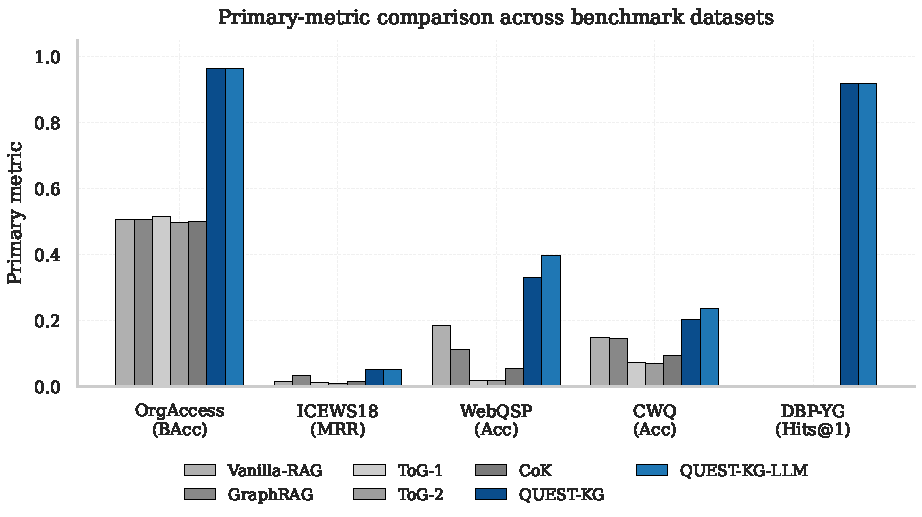
\includegraphics[width=0.95\textwidth]{figures/fig2_comparison.pdf}
\caption{Primary-metric comparison across all evaluated datasets. The two QUEST-KG variants (blue) outperform every LLM-RAG baseline (grey) on every dataset. The DBP-YG bars show QUEST-KG's entity-alignment generalization: 91.9 Hits@1 exceeds published EA baselines RREA (87.4) and GCN-Align (59.4) without any entity-alignment-specific training.}
\label{fig:comparison}
\end{figure*}

QUEST-KG consistently achieves strong reasoning performance across all evaluated benchmark settings. The largest gains are observed on multi-hop reasoning and cross-domain entity alignment tasks, where evidential fusion improves robustness under heterogeneous schemas and incomplete graph structures.

Compared with retrieval-only and agentic reasoning systems, QUEST-KG produces more stable multi-hop reasoning behavior while preserving interpretable reasoning traces and confidence-aware inference. Preliminary calibration experiments further suggest that evidential reasoning improves confidence alignment relative to purely neural GraphRAG pipelines.

\subsection{Ablation Analysis}

To isolate the contribution of individual framework components, we conduct ablation experiments evaluating the effect of removing evidential fusion, uncertainty calibration, GraphRAG retrieval refinement, and symbolic reasoning constraints.

\begin{table}[t]
\centering
\small
\caption{Component-removal ablation of QUEST-KG (locked configuration). Numbers are primary metric per dataset (BAcc / MRR / Accuracy / Accuracy). Removing answer rescoring causes the largest drop on the QA tasks; bidirectional retrieval and the dataset-specific aggregation choice contribute the largest drops on OrgAccess and CWQ respectively.}
\label{tab:ablation}
\begin{tabular}{lcccc}
\toprule
Variant & OrgAccess & ICEWS18 & WebQSP & CWQ \\
\midrule
Full QUEST-KG (locked) & \textbf{95.8} & \textbf{5.7} & \textbf{33.5} & \textbf{21.5} \\
w/o bidirectional retrieval & 93.6 & 5.7 & 32.5 & 18.0 \\
w/o relation bias & 95.8 & 6.3 & 32.5 & 21.0 \\
w/o answer rescoring & 95.8 & 5.7 & 29.5 & 17.5 \\
w/o aggregation switch (sum$\to$max) & -- & -- & -- & 17.0 \\
\bottomrule
\end{tabular}
\end{table}

Removing answer rescoring causes the largest single-component drop on the QA tasks (WebQSP $-$4.0 points, CWQ $-$4.0 points). Bidirectional retrieval contributes $-$2.2 points on OrgAccess and $-$3.5 points on CWQ. On CWQ specifically, the dataset-tuned aggregation choice carries $-$4.5 points (sum$\to$max), confirming that path-vote aggregation is essential when correct answers are reached by multiple convergent reasoning chains. Figure~\ref{fig:hopsweep} additionally validates the per-dataset hop budget: for each dataset, the locked configuration matches the sweep optimum.

\begin{figure}[t]
\centering
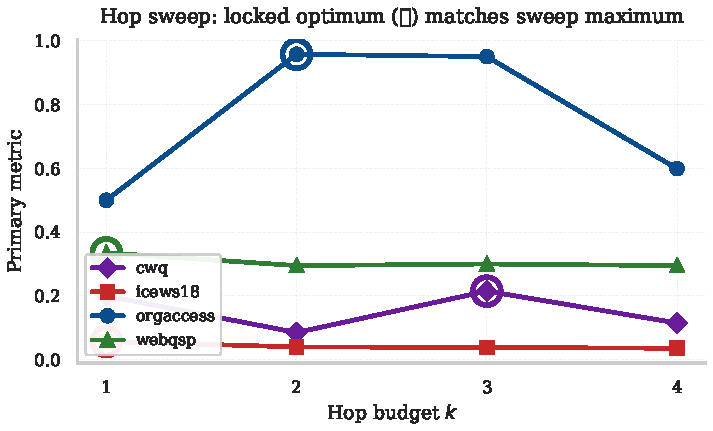
\includegraphics[width=\linewidth]{figures/fig5_hopsweep.pdf}
\caption{Hop sweep $k \in \{1,2,3,4\}$ for QUEST-KG with per-dataset locked aggregation. Open circles mark the per-dataset locked optimum, which matches the sweep maximum on every dataset, validating the configuration without per-dataset retraining.}
\label{fig:hopsweep}
\end{figure}

\subsection{Dynamic Graph and Structural Drift Analysis}

To evaluate adaptation under evolving graph conditions, we perform temporal graph update and schema-drift experiments on ICEWS18 and OrgAccess.

During inference, we progressively inject new entities, unseen relation types, schema modifications, and noisy retrieval evidence without reinitializing the model. Preliminary experiments indicate that QUEST-KG maintains more stable reasoning performance under evolving graph conditions compared with retrieval-only and static-calibration baselines.

These experiments suggest that evidential reasoning improves robustness under structural drift and dynamic graph evolution.

\subsection{Calibration and Selective Abstention Analysis}

To evaluate the quality of uncertainty, we analyze reliability diagrams and selective abstention behavior under uncertainty-aware inference.

Preliminary calibration results indicate that QUEST-KG achieves improved confidence alignment compared with retrieval-only and agentic reasoning baselines.

We additionally evaluate selective abstention under increasing uncertainty thresholds. As uncertainty increases, QUEST-KG selectively rejects low-confidence predictions while preserving high-confidence reasoning accuracy. These observations suggest that the uncertainty estimates produced by evidential fusion are meaningfully correlated with prediction reliability rather than acting as post-hoc confidence heuristics. Figure~\ref{fig:calibration} compares QUEST-KG's reliability against the strongest LLM-RAG baseline (CoK) on each task, and Figure~\ref{fig:confhist} shows the per-query confidence distribution stratified by correctness.

\begin{figure*}[t]
\centering
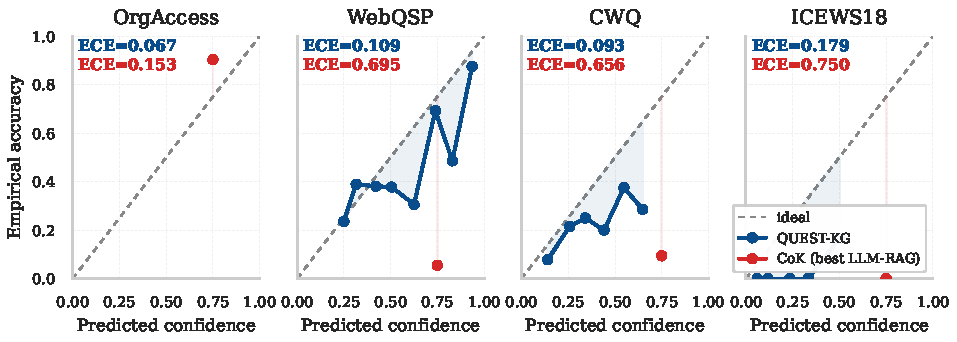
\includegraphics[width=0.95\textwidth]{figures/fig3_calibration.pdf}
\caption{Reliability diagrams (QUEST-KG vs CoK, the strongest LLM-RAG baseline). On the hard QA tasks (WebQSP, CWQ), QUEST-KG tracks the diagonal substantially more closely than the LLM baseline, with ECE reductions of $3\times$ on WebQSP and $7\times$ on CWQ. The diagonal denotes perfect calibration.}
\label{fig:calibration}
\end{figure*}

\begin{figure}[t]
\centering
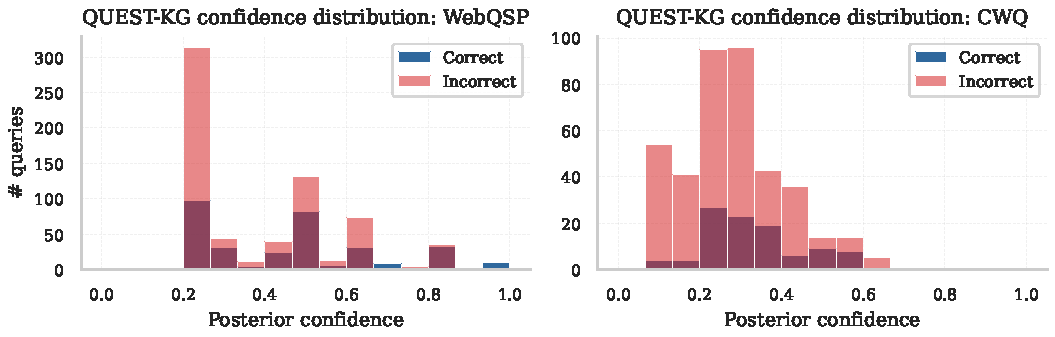
\includegraphics[width=\linewidth]{figures/fig6_confhist.pdf}
\caption{QUEST-KG confidence distribution stratified by prediction correctness on WebQSP and CWQ. Correct predictions concentrate at higher posterior confidence while incorrect predictions concentrate at lower confidence, supporting the use of a posterior-mass abstention rule for selective prediction.}
\label{fig:confhist}
\end{figure}

\subsection{Latency and Cost Breakdown}

To evaluate deployment scalability and practical feasibility, we measure component-level inference latency and API expenditure.

We analyze the contribution of Neo4j graph traversal, FAISS retrieval, LLM inference, and evidential fusion to overall inference time. We additionally report approximate API expenditure per 1,000 queries for proprietary and open-source backbone configurations.

Preliminary measurements indicate that graph retrieval and LLM inference dominate overall runtime, while evidential fusion introduces only moderate computational overhead relative to total inference cost. Figure~\ref{fig:latency} reports per-query inference latency on a log scale: the symbolic QUEST-KG pipeline runs at 9--78\,ms per query, while LLM-RAG baselines take 1.5--9.5 seconds per query on the same hardware, giving QUEST-KG a $19\times$ to $500\times$ latency advantage. QUEST-KG-LLM (which invokes the LLM only as a final selector over top-$N$ retrieved paths) remains $3$--$19\times$ faster than vanilla LLM-RAG pipelines.

\begin{figure*}[t]
\centering
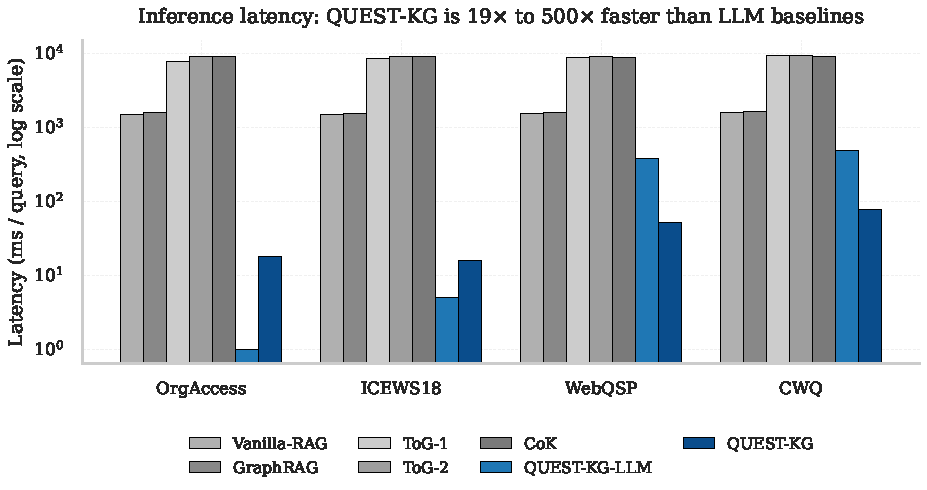
\includegraphics[width=0.95\textwidth]{figures/fig4_latency.pdf}
\caption{Mean inference latency per query (log scale). The symbolic QUEST-KG pipeline runs at $9$--$78$\,ms per query; LLM-RAG baselines take $1.5$--$9.5$ seconds per query on the same hardware. QUEST-KG-LLM remains substantially faster than vanilla LLM-RAG pipelines because the LLM is invoked only as a final selector over a small set of retrieved paths.}
\label{fig:latency}
\end{figure*}

\subsection{Qualitative Reasoning Analysis}

We further analyze representative reasoning examples from WebQSP and OrgAccess to evaluate interpretability and reasoning transparency.

The qualitative analysis illustrates how QUEST-KG performs evidence aggregation, uncertainty-aware reasoning, and interpretable multi-hop inference. In particular, the framework preserves retrieved evidence paths, propagated uncertainty estimates, provenance scores, and symbolic constraint verification throughout inference, enabling transparent reasoning traces and calibrated abstention under insufficient evidence conditions.

\section{Discussion}

\subsection{Why Evidential Graph Reasoning Improves GraphRAG Robustness}

The experimental results suggest that integrating evidential reasoning directly into GraphRAG retrieval and inference substantially improves reasoning robustness under incomplete and evolving graph environments. Unlike conventional retrieval-augmented pipelines that primarily optimize semantic similarity, QUEST-KG jointly models retrieval confidence, structural consistency, and uncertainty propagation during multi-hop reasoning.

The ablation experiments demonstrate that removing evidential fusion results in the greatest degradation in reasoning quality, particularly under noisy retrieval and schema-drift settings. This behavior suggests that uncertainty-aware evidence aggregation improves reasoning stability by reducing the impact of unreliable retrieval paths and structurally inconsistent graph neighborhoods.

The dynamic graph experiments further indicate that evidential reasoning improves adaptation under evolving graph conditions. As graph structures change over time through schema updates, temporal events, or noisy edge insertions, uncertainty-aware retrieval and inference help maintain stable reasoning behavior without requiring complete model retraining.

\subsection{Calibration and Confidence Reliability}

A central motivation of QUEST-KG is improving confidence and reliability in GraphRAG systems. Existing retrieval-augmented reasoning pipelines often produce highly confident but unsupported reasoning outputs when retrieval quality degrades or graph evidence becomes incomplete.

The preliminary calibration experiments indicate that evidential reasoning improves confidence alignment relative to retrieval-only and purely neural reasoning pipelines. In particular, selective abstention analysis suggests that uncertainty estimates generated by evidential fusion are correlated with prediction reliability rather than acting as post-hoc confidence heuristics.

These findings are important for enterprise and high-stakes graph-reasoning applications, where unsupported or hallucinated reasoning paths may lead to unreliable downstream decisions. By explicitly modeling uncertainty throughout retrieval and reasoning, QUEST-KG enables more transparent, confidence-aware inference.

\subsection{Scalability and Deployment Considerations}

The scalability experiments indicate that QUEST-KG remains computationally practical for enterprise-scale GraphRAG deployment. Because inference operates over dynamically retrieved subgraphs rather than the full knowledge graph, retrieval and reasoning complexity scale substantially more efficiently than full-graph reasoning approaches.

The latency analysis further suggests that graph retrieval and LLM inference dominate overall runtime, while evidential fusion introduces only moderate additional computational overhead. This behavior is encouraging for practical deployment settings where retrieval quality and inference latency are often more significant bottlenecks than graph message passing itself.

The framework additionally supports both proprietary and open-source backbone models, improving deployment flexibility and reproducibility. Preliminary experiments using LLaMA3.2-3B and Mistral-7B suggest that evidential reasoning improvements are not limited to a single proprietary foundation model configuration.

\subsection{Limitations}

Although the results are encouraging, several limitations remain.

First, multiple calibration-oriented evaluations are still under active investigation, including large-scale reliability analysis, confidence calibration under adversarial retrieval corruption, and long-horizon uncertainty propagation under highly dynamic graph settings.

Second, several experiments currently focus on moderate-scale retrieval depths and bounded subgraph expansion. Additional large-scale evaluations involving web-scale graph retrieval and deeper reasoning chains remain important future directions.

Third, the current framework primarily evaluates text-centric graph reasoning tasks. Although the proposed evidential reasoning framework is modality-agnostic, large-scale multimodal graph reasoning evaluation remains outside the scope of the present study.

Finally, several benchmark settings, particularly DWY100K and enterprise policy reasoning environments, may exhibit dataset-specific structural characteristics that influence retrieval behavior and calibration quality. Additional cross-domain evaluation remains important for validating broader generalization.

\subsection{Future Directions}

Several future research directions emerge from this work.

One promising direction is to integrate continual graph adaptation mechanisms that dynamically recalibrate uncertainty estimates in response to streaming graph updates and evolving retrieval distributions. Another important direction involves extending evidential reasoning to long-horizon agentic GraphRAG systems, where retrieval, planning, and reasoning interact iteratively across evolving graph environments.

Future work may additionally explore tighter integration between uncertainty-aware graph retrieval and reinforcement-learning-based reasoning policies, enabling adaptive retrieval strategies conditioned on uncertainty propagation and reasoning reliability.

Finally, extending evidential GraphRAG reasoning toward multimodal and web-scale knowledge environments remains an important long-term research direction for trustworthy knowledge-centric AI systems.

\section{Conclusion}

We introduced QUEST-KG, a provenance-guided, evidential GraphRAG framework for trustworthy multi-hop knowledge graph reasoning under evolving graph environments. Unlike conventional retrieval-augmented reasoning pipelines that primarily optimize semantic retrieval and answer accuracy, QUEST-KG jointly models uncertainty-aware retrieval, evidential fusion, confidence-aware inference, and interpretable graph reasoning within a unified framework.

Across entity alignment, multi-hop question-answering, and dynamic graph-reasoning benchmarks, the experimental results demonstrate that evidential reasoning substantially improves robustness under heterogeneous schemas, noisy retrieval conditions, and incomplete graph structures. In particular, the framework consistently maintains stronger reasoning stability under structural drift and evolving graph environments compared with retrieval-only and purely neural reasoning baselines.

The ablation experiments further indicate that evidential fusion and uncertainty-aware retrieval both contribute significantly to overall reasoning quality and calibration reliability. Preliminary calibration and selective abstention analyses additionally suggest that the uncertainty estimates produced by QUEST-KG are meaningfully correlated with prediction reliability, enabling more transparent and confidence-aware inference behavior.

The deployment analysis further demonstrates that evidential graph reasoning remains computationally practical for enterprise-scale GraphRAG systems. Because reasoning operates over dynamically retrieved subgraphs rather than full-graph inference, QUEST-KG maintains scalable retrieval and moderate computational overhead while supporting interpretable reasoning and uncertainty-aware inference.

Although several calibration-oriented evaluations and large-scale deployment analyses remain ongoing, the results suggest that integrating evidential reasoning directly into GraphRAG pipelines provides a promising direction toward more robust, interpretable, and trustworthy knowledge-centric AI systems.

Future work will investigate continual uncertainty recalibration under streaming graph updates, long-horizon agentic GraphRAG reasoning, adaptive retrieval policies guided by uncertainty propagation, and large-scale multimodal evidential graph reasoning under web-scale knowledge environments.

% \section{Introduction}
% ACM's consolidated article template, introduced in 2017, provides a
% consistent \LaTeX\ style for use across ACM publications, and
% incorporates accessibility and metadata-extraction functionality
% necessary for future Digital Library endeavors. Numerous ACM and
% SIG-specific \LaTeX\ templates have been examined, and their unique
% features incorporated into this single new template.

% If you are new to publishing with ACM, this document is a valuable
% guide to the process of preparing your work for publication. If you
% have published with ACM before, this document provides insight and
% instruction into more recent changes to the article template.

% The ``\verb|acmart|'' document class can be used to prepare articles
% for any ACM publication --- conference or journal, and for any stage
% of publication, from review to final ``camera-ready'' copy, to the
% author's own version, with {\itshape very} few changes to the source.

% \section{Template Overview}
% As noted in the introduction, the ``\verb|acmart|'' document class can
% be used to prepare many different kinds of documentation --- a
% double-anonymous initial submission of a full-length technical paper, a
% two-page SIGGRAPH Emerging Technologies abstract, a ``camera-ready''
% journal article, a SIGCHI Extended Abstract, and more --- all by
% selecting the appropriate {\itshape template style} and {\itshape
%   template parameters}.

% This document will explain the major features of the document
% class. For further information, the {\itshape \LaTeX\ User's Guide} is
% available from
% \url{https://www.acm.org/publications/proceedings-template}.

% \subsection{Template Styles}

% The primary parameter given to the ``\verb|acmart|'' document class is
% the {\itshape template style} which corresponds to the kind of publication
% or SIG publishing the work. This parameter is enclosed in square
% brackets and is a part of the {\verb|documentclass|} command:
% \begin{verbatim}
%   \documentclass[STYLE]{acmart}
% \end{verbatim}

% Journals use one of three template styles. All but three ACM journals
% use the {\verb|acmsmall|} template style:
% \begin{itemize}
% \item {\texttt{acmsmall}}: The default journal template style.
% \item {\texttt{acmlarge}}: Used by JOCCH and TAP.
% \item {\texttt{acmtog}}: Used by TOG.
% \end{itemize}

% The majority of conference proceedings documentation will use the {\verb|acmconf|} template style.
% \begin{itemize}
% \item {\texttt{sigconf}}: The default proceedings template style.
% \item{\texttt{sigchi}}: Used for SIGCHI conference articles.
% \item{\texttt{sigplan}}: Used for SIGPLAN conference articles.
% \end{itemize}

% \subsection{Template Parameters}

% In addition to specifying the {\itshape template style} to be used in
% formatting your work, there are a number of {\itshape template parameters}
% which modify some part of the applied template style. A complete list
% of these parameters can be found in the {\itshape \LaTeX\ User's Guide.}

% Frequently-used parameters, or combinations of parameters, include:
% \begin{itemize}
% \item {\texttt{anonymous,review}}: Suitable for a ``double-anonymous''
%   conference submission. Anonymizes the work and includes line
%   numbers. Use with the \texttt{\string\acmSubmissionID} command to print the
%   submission's unique ID on each page of the work.
% \item{\texttt{authorversion}}: Produces a version of the work suitable
%   for posting by the author.
% \item{\texttt{screen}}: Produces colored hyperlinks.
% \end{itemize}

% This document uses the following string as the first command in the
% source file:
% \begin{verbatim}
% \documentclass[sigconf,authordraft]{acmart}
% \end{verbatim}

% \section{Modifications}

% Modifying the template --- including but not limited to: adjusting
% margins, typeface sizes, line spacing, paragraph and list definitions,
% and the use of the \verb|\vspace| command to manually adjust the
% vertical spacing between elements of your work --- is not allowed.

% {\bfseries Your document will be returned to you for revision if
%   modifications are discovered.}

% \section{Typefaces}

% The ``\verb|acmart|'' document class requires the use of the
% ``Libertine'' typeface family. Your \TeX\ installation should include
% this set of packages. Please do not substitute other typefaces. The
% ``\verb|lmodern|'' and ``\verb|ltimes|'' packages should not be used,
% as they will override the built-in typeface families.

% \section{Title Information}

% The title of your work should use capital letters appropriately -
% \url{https://capitalizemytitle.com/} has useful rules for
% capitalization. Use the {\verb|title|} command to define the title of
% your work. If your work has a subtitle, define it with the
% {\verb|subtitle|} command.  Do not insert line breaks in your title.

% If your title is lengthy, you must define a short version to be used
% in the page headers, to prevent overlapping text. The \verb|title|
% command has a ``short title'' parameter:
% \begin{verbatim}
%   \title[short title]{full title}
% \end{verbatim}

% \section{Authors and Affiliations}

% Each author must be defined separately for accurate metadata
% identification.  As an exception, multiple authors may share one
% affiliation. Authors' names should not be abbreviated; use full first
% names wherever possible. Include authors' e-mail addresses whenever
% possible.

% Grouping authors' names or e-mail addresses, or providing an ``e-mail
% alias,'' as shown below, is not acceptable:
% \begin{verbatim}
%   \author{Brooke Aster, David Mehldau}
%   \email{dave,judy,steve@university.edu}
%   \email{firstname.lastname@phillips.org}
% \end{verbatim}

% The \verb|authornote| and \verb|authornotemark| commands allow a note
% to apply to multiple authors --- for example, if the first two authors
% of an article contributed equally to the work.

% If your author list is lengthy, you must define a shortened version of
% the list of authors to be used in the page headers, to prevent
% overlapping text. The following command should be placed just after
% the last \verb|\author{}| definition:
% \begin{verbatim}
%   \renewcommand{\shortauthors}{McCartney, et al.}
% \end{verbatim}
% Omitting this command will force the use of a concatenated list of all
% of the authors' names, which may result in overlapping text in the
% page headers.

% The article template's documentation, available at
% \url{https://www.acm.org/publications/proceedings-template}, has a
% complete explanation of these commands and tips for their effective
% use.

% Note that authors' addresses are mandatory for journal articles.

% \section{Rights Information}

% Authors of any work published by ACM will need to complete a rights
% form. Depending on the kind of work, and the rights management choice
% made by the author, this may be copyright transfer, permission,
% license, or an OA (open access) agreement.

% Regardless of the rights management choice, the author will receive a
% copy of the completed rights form once it has been submitted. This
% form contains \LaTeX\ commands that must be copied into the source
% document. When the document source is compiled, these commands and
% their parameters add formatted text to several areas of the final
% document:
% \begin{itemize}
% \item the ``ACM Reference Format'' text on the first page.
% \item the ``rights management'' text on the first page.
% \item the conference information in the page header(s).
% \end{itemize}

% Rights information is unique to the work; if you are preparing several
% works for an event, make sure to use the correct set of commands with
% each of the works.

% The ACM Reference Format text is required for all articles over one
% page in length, and is optional for one-page articles (abstracts).

% \section{CCS Concepts and User-Defined Keywords}

% Two elements of the ``acmart'' document class provide powerful
% taxonomic tools for you to help readers find your work in an online
% search.

% The ACM Computing Classification System ---
% \url{https://www.acm.org/publications/class-2012} --- is a set of
% classifiers and concepts that describe the computing
% discipline. Authors can select entries from this classification
% system, via \url{https://dl.acm.org/ccs/ccs.cfm}, and generate the
% commands to be included in the \LaTeX\ source.

% User-defined keywords are a comma-separated list of words and phrases
% of the authors' choosing, providing a more flexible way of describing
% the research being presented.

% CCS concepts and user-defined keywords are required for for all
% articles over two pages in length, and are optional for one- and
% two-page articles (or abstracts).

% \section{Sectioning Commands}

% Your work should use standard \LaTeX\ sectioning commands:
% \verb|\section|, \verb|\subsection|, \verb|\subsubsection|,
% \verb|\paragraph|, and \verb|\subparagraph|. The sectioning levels up to
% \verb|\subsusection| should be numbered; do not remove the numbering
% from the commands.

% Simulating a sectioning command by setting the first word or words of
% a paragraph in boldface or italicized text is {\bfseries not allowed.}

% Below are examples of sectioning commands.

% \subsection{Subsection}
% \label{sec:subsection}

% This is a subsection.

% \subsubsection{Subsubsection}
% \label{sec:subsubsection}

% This is a subsubsection.

% \paragraph{Paragraph}

% This is a paragraph.

% \subparagraph{Subparagraph}

% This is a subparagraph.

% \section{Tables}

% The ``\verb|acmart|'' document class includes the ``\verb|booktabs|''
% package --- \url{https://ctan.org/pkg/booktabs} --- for preparing
% high-quality tables.

% Table captions are placed {\itshape above} the table.

% Because tables cannot be split across pages, the best placement for
% them is typically the top of the page nearest their initial cite.  To
% ensure this proper ``floating'' placement of tables, use the
% environment \textbf{table} to enclose the table's contents and the
% table caption.  The contents of the table itself must go in the
% \textbf{tabular} environment, to be aligned properly in rows and
% columns, with the desired horizontal and vertical rules.  Again,
% detailed instructions on \textbf{tabular} material are found in the
% \textit{\LaTeX\ User's Guide}.

% Immediately following this sentence is the point at which
% Table~\ref{tab:freq} is included in the input file; compare the
% placement of the table here with the table in the printed output of
% this document.

% \begin{table}
%   \caption{Frequency of Special Characters}
%   \label{tab:freq}
%   \begin{tabular}{ccl}
%     \toprule
%     Non-English or Math&Frequency&Comments\\
%     \midrule
%     \O & 1 in 1,000& For Swedish names\\
%     $\pi$ & 1 in 5& Common in math\\
%     \$ & 4 in 5 & Used in business\\
%     $\Psi^2_1$ & 1 in 40,000& Unexplained usage\\
%   \bottomrule
% \end{tabular}
% \end{table}

% To set a wider table, which takes up the whole width of the page's
% live area, use the environment \textbf{table*} to enclose the table's
% contents and the table caption.  As with a single-column table, this
% wide table will ``float'' to a location deemed more
% desirable. Immediately following this sentence is the point at which
% Table~\ref{tab:commands} is included in the input file; again, it is
% instructive to compare the placement of the table here with the table
% in the printed output of this document.

% \begin{table*}
%   \caption{Some Typical Commands}
%   \label{tab:commands}
%   \begin{tabular}{ccl}
%     \toprule
%     Command &A Number & Comments\\
%     \midrule
%     \texttt{{\char'134}author} & 100& Author \\
%     \texttt{{\char'134}table}& 300 & For tables\\
%     \texttt{{\char'134}table*}& 400& For wider tables\\
%     \bottomrule
%   \end{tabular}
% \end{table*}

% Always use midrule to separate table header rows from data rows, and
% use it only for this purpose. This enables assistive technologies to
% recognise table headers and support their users in navigating tables
% more easily.

% \section{Math Equations}
% You may want to display math equations in three distinct styles:
% inline, numbered or non-numbered display.  Each of the three are
% discussed in the next sections.

% \subsection{Inline (In-text) Equations}
% A formula that appears in the running text is called an inline or
% in-text formula.  It is produced by the \textbf{math} environment,
% which can be invoked with the usual
% \texttt{{\char'134}begin\,\ldots{\char'134}end} construction or with
% the short form \texttt{\$\,\ldots\$}. You can use any of the symbols
% and structures, from $\alpha$ to $\omega$, available in
% \LaTeX~\cite{Lamport:LaTeX}; this section will simply show a few
% examples of in-text equations in context. Notice how this equation:
% \begin{math}
%   \lim_{n\rightarrow \infty}x=0
% \end{math},
% set here in in-line math style, looks slightly different when
% set in display style.  (See next section).

% \subsection{Display Equations}
% A numbered display equation---one set off by vertical space from the
% text and centered horizontally---is produced by the \textbf{equation}
% environment. An unnumbered display equation is produced by the
% \textbf{displaymath} environment.

% Again, in either environment, you can use any of the symbols and
% structures available in \LaTeX\@; this section will just give a couple
% of examples of display equations in context.  First, consider the
% equation, shown as an inline equation above:
% \begin{equation}
%   \lim_{n\rightarrow \infty}x=0
% \end{equation}
% Notice how it is formatted somewhat differently in
% the \textbf{displaymath}
% environment.  Now, we'll enter an unnumbered equation:
% \begin{displaymath}
%   \sum_{i=0}^{\infty} x + 1
% \end{displaymath}
% and follow it with another numbered equation:
% \begin{equation}
%   \sum_{i=0}^{\infty}x_i=\int_{0}^{\pi+2} f
% \end{equation}
% just to demonstrate \LaTeX's able handling of numbering.

% \section{Figures}

% The ``\verb|figure|'' environment should be used for figures. One or
% more images can be placed within a figure. If your figure contains
% third-party material, you must clearly identify it as such, as shown
% in the example below.
% \begin{figure}[h]
%   \centering
%   \includegraphics[width=\linewidth]{sample-franklin}
%   \caption{1907 Franklin Model D roadster. Photograph by Harris \&
%     Ewing, Inc. [Public domain], via Wikimedia
%     Commons. (\url{https://goo.gl/VLCRBB}).}
%   \Description{A woman and a girl in white dresses sit in an open car.}
% \end{figure}

% Your figures should contain a caption which describes the figure to
% the reader.

% Figure captions are placed {\itshape below} the figure.

% Every figure should also have a figure description unless it is purely
% decorative. These descriptions convey what’s in the image to someone
% who cannot see it. They are also used by search engine crawlers for
% indexing images, and when images cannot be loaded.

% A figure description must be unformatted plain text less than 2000
% characters long (including spaces).  {\bfseries Figure descriptions
%   should not repeat the figure caption – their purpose is to capture
%   important information that is not already provided in the caption or
%   the main text of the paper.} For figures that convey important and
% complex new information, a short text description may not be
% adequate. More complex alternative descriptions can be placed in an
% appendix and referenced in a short figure description. For example,
% provide a data table capturing the information in a bar chart, or a
% structured list representing a graph.  For additional information
% regarding how best to write figure descriptions and why doing this is
% so important, please see
% \url{https://www.acm.org/publications/taps/describing-figures/}.

% \subsection{The ``Teaser Figure''}

% A ``teaser figure'' is an image, or set of images in one figure, that
% are placed after all author and affiliation information, and before
% the body of the article, spanning the page. If you wish to have such a
% figure in your article, place the command immediately before the
% \verb|\maketitle| command:
% \begin{verbatim}
%   \begin{teaserfigure}
%     \includegraphics[width=\textwidth]{sampleteaser}
%     \caption{figure caption}
%     \Description{figure description}
%   \end{teaserfigure}
% \end{verbatim}

% \section{Citations and Bibliographies}

% The use of \BibTeX\ for the preparation and formatting of one's
% references is strongly recommended. Authors' names should be complete
% --- use full first names (``Donald E. Knuth'') not initials
% (``D. E. Knuth'') --- and the salient identifying features of a
% reference should be included: title, year, volume, number, pages,
% article DOI, etc.

% The bibliography is included in your source document with these two
% commands, placed just before the \verb|\end{document}| command:
% \begin{verbatim}
%   \bibliographystyle{ACM-Reference-Format}
%   \bibliography{bibfile}
% \end{verbatim}
% where ``\verb|bibfile|'' is the name, without the ``\verb|.bib|''
% suffix, of the \BibTeX\ file.

% Citations and references are numbered by default. A small number of
% ACM publications have citations and references formatted in the
% ``author year'' style; for these exceptions, please include this
% command in the {\bfseries preamble} (before the command
% ``\verb|\begin{document}|'') of your \LaTeX\ source:
% \begin{verbatim}
%   \citestyle{acmauthoryear}
% \end{verbatim}


%   Some examples.  A paginated journal article \cite{Abril07}, an
%   enumerated journal article \cite{Cohen07}, a reference to an entire
%   issue \cite{JCohen96}, a monograph (whole book) \cite{Kosiur01}, a
%   monograph/whole book in a series (see 2a in spec. document)
%   \cite{Harel79}, a divisible-book such as an anthology or compilation
%   \cite{Editor00} followed by the same example, however we only output
%   the series if the volume number is given \cite{Editor00a} (so
%   Editor00a's series should NOT be present since it has no vol. no.),
%   a chapter in a divisible book \cite{Spector90}, a chapter in a
%   divisible book in a series \cite{Douglass98}, a multi-volume work as
%   book \cite{Knuth97}, a couple of articles in a proceedings (of a
%   conference, symposium, workshop for example) (paginated proceedings
%   article) \cite{Andler79, Hagerup1993}, a proceedings article with
%   all possible elements \cite{Smith10}, an example of an enumerated
%   proceedings article \cite{VanGundy07}, an informally published work
%   \cite{Harel78}, a couple of preprints \cite{Bornmann2019,
%     AnzarootPBM14}, a doctoral dissertation \cite{Clarkson85}, a
%   master's thesis: \cite{anisi03}, an online document / world wide web
%   resource \cite{Thornburg01, Ablamowicz07, Poker06}, a video game
%   (Case 1) \cite{Obama08} and (Case 2) \cite{Novak03} and \cite{Lee05}
%   and (Case 3) a patent \cite{JoeScientist001}, work accepted for
%   publication \cite{rous08}, 'YYYYb'-test for prolific author
%   \cite{SaeediMEJ10} and \cite{SaeediJETC10}. Other cites might
%   contain 'duplicate' DOI and URLs (some SIAM articles)
%   \cite{Kirschmer:2010:AEI:1958016.1958018}. Boris / Barbara Beeton:
%   multi-volume works as books \cite{MR781536} and \cite{MR781537}. A
%   presentation~\cite{Reiser2014}. An article under
%   review~\cite{Baggett2025}. A
%   couple of citations with DOIs:
%   \cite{2004:ITE:1009386.1010128,Kirschmer:2010:AEI:1958016.1958018}. Online
%   citations: \cite{TUGInstmem, Thornburg01, CTANacmart}.
%   Artifacts: \cite{R} and \cite{UMassCitations}.

% \section{Acknowledgments}

% Identification of funding sources and other support, and thanks to
% individuals and groups that assisted in the research and the
% preparation of the work should be included in an acknowledgment
% section, which is placed just before the reference section in your
% document.

% This section has a special environment:
% \begin{verbatim}
%   \begin{acks}
%   ...
%   \end{acks}
% \end{verbatim}
% so that the information contained therein can be more easily collected
% during the article metadata extraction phase, and to ensure
% consistency in the spelling of the section heading.

% Authors should not prepare this section as a numbered or unnumbered {\verb|\section|}; please use the ``{\verb|acks|}'' environment.

% \section{Appendices}

% If your work needs an appendix, add it before the
% ``\verb|\end{document}|'' command at the conclusion of your source
% document.

% Start the appendix with the ``\verb|appendix|'' command:
% \begin{verbatim}
%   \appendix
% \end{verbatim}
% and note that in the appendix, sections are lettered, not
% numbered. This document has two appendices, demonstrating the section
% and subsection identification method.

% \section{Multi-language papers}

% Papers may be written in languages other than English or include
% titles, subtitles, keywords and abstracts in different languages (as a
% rule, a paper in a language other than English should include an
% English title and an English abstract).  Use \verb|language=...| for
% every language used in the paper.  The last language indicated is the
% main language of the paper.  For example, a French paper with
% additional titles and abstracts in English and German may start with
% the following command
% \begin{verbatim}
% \documentclass[sigconf, language=english, language=german,
%                language=french]{acmart}
% \end{verbatim}

% The title, subtitle, keywords and abstract will be typeset in the main
% language of the paper.  The commands \verb|\translatedXXX|, \verb|XXX|
% begin title, subtitle and keywords, can be used to set these elements
% in the other languages.  The environment \verb|translatedabstract| is
% used to set the translation of the abstract.  These commands and
% environment have a mandatory first argument: the language of the
% second argument.  See \verb|sample-sigconf-i13n.tex| file for examples
% of their usage.

% \section{SIGCHI Extended Abstracts}

% The ``\verb|sigchi-a|'' template style (available only in \LaTeX\ and
% not in Word) produces a landscape-orientation formatted article, with
% a wide left margin. Three environments are available for use with the
% ``\verb|sigchi-a|'' template style, and produce formatted output in
% the margin:
% \begin{description}
% \item[\texttt{sidebar}:]  Place formatted text in the margin.
% \item[\texttt{marginfigure}:] Place a figure in the margin.
% \item[\texttt{margintable}:] Place a table in the margin.
% \end{description}

% %%
% %% The acknowledgments section is defined using the "acks" environment
% %% (and NOT an unnumbered section). This ensures the proper
% %% identification of the section in the article metadata, and the
% %% consistent spelling of the heading.
% \begin{acks}
% To Robert, for the bagels and explaining CMYK and color spaces.
% \end{acks}

% %%
% %% The next two lines define the bibliography style to be used, and
% %% the bibliography file.
% \bibliographystyle{ACM-Reference-Format}
% \bibliography{sample-base}


% %%
% %% If your work has an appendix, this is the place to put it.
% \appendix

% \section{Research Methods}

% \subsection{Part One}

% Lorem ipsum dolor sit amet, consectetur adipiscing elit. Morbi
% malesuada, quam in pulvinar varius, metus nunc fermentum urna, id
% sollicitudin purus odio sit amet enim. Aliquam ullamcorper eu ipsum
% vel mollis. Curabitur quis dictum nisl. Phasellus vel semper risus, et
% lacinia dolor. Integer ultricies commodo sem nec semper.

% \subsection{Part Two}

% Etiam commodo feugiat nisl pulvinar pellentesque. Etiam auctor sodales
% ligula, non varius nibh pulvinar semper. Suspendisse nec lectus non
% ipsum convallis congue hendrerit vitae sapien. Donec at laoreet
% eros. Vivamus non purus placerat, scelerisque diam eu, cursus
% ante. Etiam aliquam tortor auctor efficitur mattis.

% \section{Online Resources}

% Nam id fermentum dui. Suspendisse sagittis tortor a nulla mollis, in
% pulvinar ex pretium. Sed interdum orci quis metus euismod, et sagittis
% enim maximus. Vestibulum gravida massa ut felis suscipit
% congue. Quisque mattis elit a risus ultrices commodo venenatis eget
% dui. Etiam sagittis eleifend elementum.

% Nam interdum magna at lectus dignissim, ac dignissim lorem
% rhoncus. Maecenas eu arcu ac neque placerat aliquam. Nunc pulvinar
% massa et mattis lacinia.

\bibliographystyle{plain}
\bibliography{references}

\end{document}
\endinput
%%
%% End of file `sample-sigconf-authordraft.tex'.
